\section{2D system simulation}

\subsection{System overview}
The system presented is a Multiple Input Multiple Output (MIMO) system, such that in this case there are 4 inputs and 2 outputs. 

The 2 outputs that it is needed to control are:
\begin{itemize}
	\item Drone's antenna angle ($\theta_{d}$)
	\item Groundstation's antenna angle ($\theta_{gs}$)
\end{itemize}

The system's inputs are as follows:
\begin{itemize}
	\item Drone's antenna angle ($\theta_{d}$)
	\item Groundstation's antenna angle ($\theta_{gs}$)
	\item Drone position ($x_{drone},y_{drone}$)
	\item Groundstation position ($x_{gs},y_{gs}$)
\end{itemize}

\begin{figure}
	\centering
	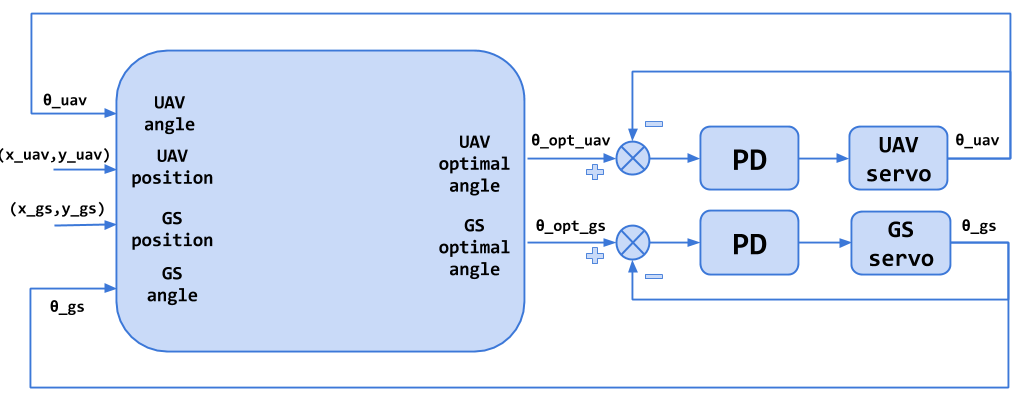
\includegraphics[scale=0.42]{figures/2d_system.png}
	\caption{2D sytem overview}
	\label{fig:2d_system}
\end{figure}

\subsection{Optimal angle}
The first block of the system takes the inputs above and computes the optimal angles for the groundstation and drone antenna, such that a strong communication link is achieved.  

% \begin{figure}
% 	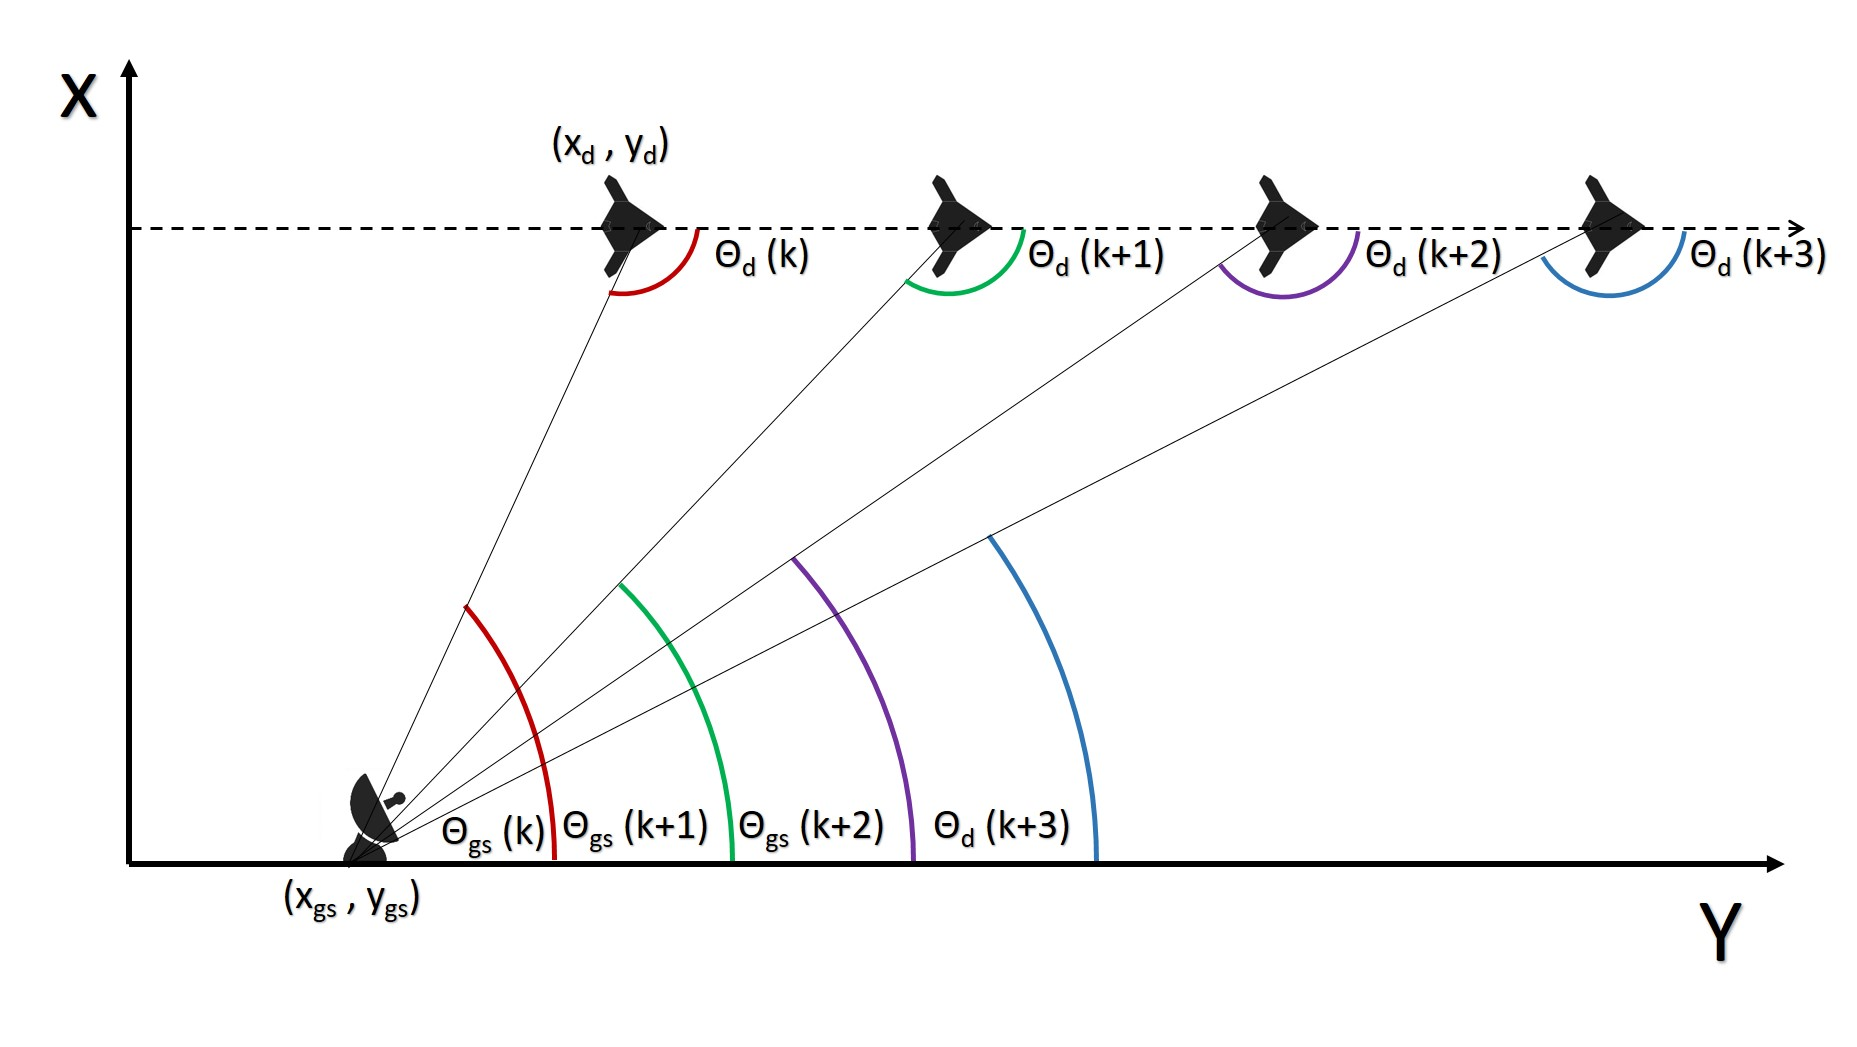
\includegraphics[scale=1]{\fig\drone_gs_ex.jpg}
% 	\caption{Example of a drone-gs with 3 angles}
% 	\label{fig:drone_gs_ex}
% \end{figure}


% \subsection{}